% Keep the expanded appendix readable without changing the protected main-paper layout.
\renewcommand{\topfraction}{0.95}
\renewcommand{\dbltopfraction}{0.95}
\renewcommand{\textfraction}{0.05}
\renewcommand{\floatpagefraction}{0.85}
\renewcommand{\dblfloatpagefraction}{0.85}
\setcounter{topnumber}{4}
\setcounter{dbltopnumber}{4}
\setcounter{totalnumber}{8}

\FloatBarrier
\section{Protocol Details}
\label{app:protocol}

\paragraph{Cost-aware audit protocol.}
Table~\ref{tab:supp-cost-aware-audit-protocol} summarizes the protocol used throughout this study. Because the audited object is a scaffolded inference procedure, a row should not be promoted from diagnostic evidence to method evidence unless the input contract, output schema, scorer, failure accounting and cost trace are matched.

\begin{table}[!htbp]
\centering
\small
\setlength{\tabcolsep}{3pt}
\begin{tabular}{@{}p{0.75cm}p{1.8cm}p{4.4cm}@{}}
\toprule
\textbf{Step} & \textbf{Check} & \textbf{Audit rule} \\
\midrule
1 & Scope & Name the scaffold, input field, answer contract, scorer and non-claims before comparing methods. \\
2 & Match rows & Run the scaffold and alternatives on identical instances; separate development, fixed-pipeline and split-validity evidence. \\
3 & Cheap route & Include deterministic code, retrieval/reranking, SLM workers, direct LLM and RLM only where each is natural for the operation. \\
4 & Cost/failures & Record per-example cost, timeout/error rows, retry/stop rules and attempted-cost lower bounds. \\
5 & Confounds & Add finalizer, schema, same-operator, wrong-family, repeatability and trace probes when results could be harness artifacts. \\
6 & Claims & Mark rows as confirmed, diagnostic, smoke, proxy or future; report falsifiers and candidate-positive regimes separately. \\
\bottomrule
\end{tabular}
\caption{Cost-aware audit protocol used in this study. Standard RLM is compared only after cheaper operation-matched mechanisms receive the same instances, answer contract, scorer, cost logging and failure accounting.}
\label{tab:supp-cost-aware-audit-protocol}
\end{table}

\paragraph{Role-based model coverage.}
The primary panel assigns models to deployment roles rather than constructing a broad leaderboard: Gemini~2.5~Flash controls the logged standard RLM and supplies direct frontier inference, Gemma~4~26B-A4B supplies SLM worker paths and GPT-4o-mini controls the short T-NLP LLM+SLM route. GPT-5 is used for the T-STRUCT frontier-controller exception and a CD-45 controller sensitivity. Many central alternatives are deterministic or structural so the unresolved breadth question is same-contract coverage of stronger RLM-family systems rather than additional direct-LLM columns.

That stronger-family evidence includes frozen-manifest adapter pressure tests, matched standard-unlabeled smokes, the CD-15 repeatability study and CD-45 same-operator-library diagnostics. The unmodified public $\lambda$-RLM repository attempts all 15 frozen CD-15 IDs with its published Qwen3-8B settings and reaches 8/15 exact with two declared timeouts. MIT OASYS's official \texttt{rlm-qwen3-30b-a3b-v0.1} post-trained policy reaches 10/15 exact with one timeout through the canonical \texttt{rlm} harness and model-card Oolong settings. The $\lambda$ row is official-code cross-task evidence rather than an original-paper reproduction; rankable official SRLM and same-contract RAH rows remain unavailable.

Controller-freshness and compatibility checks are reported separately from family parity. Table~\ref{tab:supp-protocol-caps} gives the contracts for the complete central and sensitivity rows; these checks do not constitute full official SRLM/$\lambda$-RLM/RAH benchmark parity.

\begin{table*}[!t]
\centering
\small
\setlength{\tabcolsep}{3pt}
\begin{tabular}{@{}L{0.24\linewidth}L{0.20\linewidth}L{0.12\linewidth}L{0.35\linewidth}@{}}
\toprule
\textbf{Slice / row} & \textbf{RLM controller} & \textbf{Row cap} & \textbf{Interpretation} \\
\midrule
Oolong CD-45 central & Gemini~2.5 Flash & 360s & Main standard-\texttt{rlms} row. \\
Oolong CD-15 repeats & Gemini~2.5 Flash & 360s & Repeatability diagnostic over a frozen subset. \\
Oolong CD-15 official trained policy & Qwen3-30B-A3B + official LoRA & 1500s & Canonical-harness, same-contract diagnostic; one timeout is scored incorrect. \\
Oolong CD-45 same-operator RLM & Gemini~2.5 Flash & 360s & Standard-\texttt{rlms} custom-tool diagnostic, not official SRLM/$\lambda$-RLM. \\
Oolong CD-45 controller sensitivity & GPT-5 & 240s & Controller+stability sensitivity, not pure controller ablation. \\
Oolong CD-45 GPT-5.6 complete & GPT-5.6 Luna & 360s & Current-controller sensitivity; complete strict-stop row, not official SRLM/$\lambda$-RLM/RAH. \\
Oolong CD-15 official $\lambda$ code & Qwen3-8B & 1800s & Complete unmodified-repository cross-task row; 15/15 attempted, 13 completed, 8 exact. \\
LB2 $>$500k smoke & Gemini~2.5 Flash & 480s & Stop-rule feasibility smoke, not stable ranking. \\
\bottomrule
\end{tabular}
\caption{Protocol caps for complete claim-central and sensitivity rows. The rows answer different questions and should not be merged as pure model swaps.}
\label{tab:supp-protocol-caps}
\end{table*}

\paragraph{Cost accounting.}
RLM cost aggregates controller program generation, recursive or child-query execution and final answer extraction. Direct LLM/SLM baselines are single-call unless retrieval-augmented. Fixed operators have zero marginal LLM cost but not zero engineering cost; hybrid pipelines such as T-STRUCT include their SLM extraction calls. Current RLM cost averages are successful-completion costs from row-level logged prediction/cost/error files; not every central RLM row retains a full raw generated-program/provider-payload trajectory. The release includes an attempted-cost audit script and JSON artifact that scan local \texttt{model\_calls*.jsonl} files for official-RLM completion rows rather than any one headline run. Across those 85 logged attempt rows, 76 completed rows record \$1.289 total cost while 9 failed timeout/error rows record zero captured usage/cost. Thus the local logs support a recorded attempted-cost lower bound across archived official-RLM model-call traces but they cannot reconcile to a single Oolong/T-MIXED headline denominator or reconstruct provider-side billing for failed partial scaffold calls whose usage was not returned.

Because person-hour estimates are unavailable, we report a deterministic audit of implementation surface. The complete released typed-route package spans four source files and 2,017 physical lines (1,793 nonblank) including the SLM labeler, typed aggregation kernel, natural-language schema parser, standard-RLM tool wrappers, command-line interfaces, caching, tracing and analysis support. The release declares schemas for six families and five answer types. Three families appear as controlled families in the main paper; the others support supplement-only diagnostics or public anchoring. The standard-RLM diagnostic exposes five atomic/schema tools and one optional convenience solver. These counts are an auditable upper bound on the released implementation surface, not a minimal runtime kernel or a measure of human engineering time, maintenance burden or total cost of ownership.

We also parameterize the unmeasured one-time implementation cost instead of treating it as zero. On SU-150, the observed successful-completion API-cost difference is \$0.022041 per case; amortizing assumed one-time budgets of \$100, \$1,000 and \$10,000 from API savings alone requires 4,538, 45,371 and 453,704 cases when the ratio is computed from unrounded costs and rounded up to the next whole case. On VC-45, the corresponding difference is \$0.018377 and the thresholds are 5,442, 54,416 and 544,158 cases under the same rule. These are deployment-volume sensitivities, not estimates of actual labor or maintenance. They omit failed-call billing, latency value, reliability and future model-price changes; SU-150 also reuses prior windows while VC-45 is source-corpus transfer without document-level independence.

A deterministic cost-sensitivity audit reconciles the stored result files. T-STRUCT's roughly 99$\times$ gap is a deployed-configuration comparison: GPT-5-backed standard RLM costs \$0.019826/example on the stored run while the Gemma extraction plus fixed aggregation route is estimated at \$0.0002/example. It is not a pure matched-model estimate of scaffold overhead. For the Oolong $N=30$ pilot, the corrected SLM-labeler token-trace price is \$0.007257 versus \$0.255676 for RLM (35.2$\times$); the older pre-patch SLM estimate was \$0.103732 and still leaves RLM 2.46$\times$ more expensive. On the Oolong $N=120$ public-contract run, RLM costs \$2.688340 versus \$0.658995 for SLM+typed (4.08$\times$). The larger $N=150$ fixed-pipeline replication gives \$4.144901 versus \$0.838777 (4.94$\times$ captured successful-completion cost). Exact prices may change, but the reported cost comparisons survive the disclosed sensitivity checks within their stated deployment scope.

\FloatBarrier
\section{Diagnostic Validity Controls}
\label{app:diagnostics}

\begin{table*}[!t]
\centering
\small
\setlength{\tabcolsep}{4pt}
\begin{tabular}{@{}p{6.0cm}rrrr@{}}
\toprule
\textbf{Method} & \textbf{Exact} & \textbf{Acc.} & \textbf{Cost} & \textbf{Invalid ex.} \\
\midrule
BM25 + Gemma reader & 8/30 & 26.7\% & \$0.0355 & 3 \\
BM25 + Gemini reader & 11/30 & 36.7\% & \$0.1588 & 2 \\
BM25 + Gemma rerank + Gemini & 12/30 & 40.0\% & \$0.1863 & 2 \\
\bottomrule
\end{tabular}
\caption{Balanced LongBench-v2 train-split $>$500k-character retrieval/rerank diagnostic ($N=30$, five examples from each domain, seed 20260714). All rows use local BM25 over the full context and three answer-order votes. The rerank row applies Gemma to score 24 BM25 candidates before Gemini reads the selected excerpts. This is an over-window alternative diagnostic, not a same-row RLM-family comparison.}
\label{tab:supp-lb2-over500k-rerank}
\end{table*}

\begin{table*}[!t]
\centering
\small
\setlength{\tabcolsep}{4pt}
\begin{tabular}{@{}p{6.0cm}rrrr@{}}
\toprule
\textbf{Method} & \textbf{Exact} & \textbf{Acc.} & \textbf{Cost} & \textbf{Errors} \\
\midrule
Standard \texttt{rlms} & 1/6 & 16.7\% & \$0.4698 & 1 \\
BM25 + Gemma reader & 1/6 & 16.7\% & \$0.0065 & 0 \\
BM25 + Gemini reader & 2/6 & 33.3\% & \$0.0284 & 0 \\
BM25 + Gemma rerank + Gemini & 2/6 & 33.3\% & \$0.0326 & 0 \\
\bottomrule
\end{tabular}
\caption{Same-row standard-\texttt{rlms} smoke on the balanced LongBench-v2 train-split $>$500k-character manifest. The six rows are the shortest eligible context in each balanced domain. This is a stop-rule feasibility check, not a full $N=30$ ranking.}
\label{tab:supp-lb2-over500k-rlm-smoke}
\end{table*}

\Needspace{6\baselineskip}
The balanced diagnostic covers Code Repository Understanding, Long In-context Learning, Long Structured Data Understanding, Long-dialogue History Understanding, Multi-Document QA and Single-Document QA. The strongest row, BM25+Gemma-rerank+Gemini, reaches 3/5 on code, 2/5 on in-context learning, 2/5 on structured data, 1/5 on dialogue, 3/5 on multi-document QA and 1/5 on single-document QA. Reranking changes three rows and improves only one net example over BM25+Gemini. We therefore use the result to calibrate the over-window boundary: cheap retrieval/reranking is a necessary comparison for RLM but this particular route does not close the extreme-context region.

\paragraph{Multiple-choice position control.}
On the LongBench-v2 Academic QA discovery set ($N=50$), canonical BM25 predicts option A on 68\% of rows while only 18\% of gold answers are A. Rotating answer-order priming improves the pooled $N=94$ comparison ($p=0.015$) but not the held-out $N=44$ slice alone ($p=1.0$). Single-call accuracy was not separately measured, so this remains a format-validity diagnostic rather than evidence for a retrieval or RLM ranking.

\paragraph{Post-hoc dense-rerank sensitivity.}
On the attempted-$N=49$ BrowseComp-Plus replication rows, a same-row post-hoc route reranks 64 BM25 candidates with Qwen3-Embedding-8B before the same Qwen answer model and Gemma judge. The hybrid scores 20/49 at \$0.516 versus 22/49 at \$0.509 for matched BM25 replay and 35/49 for RLM; RLM--hybrid is +30.6 points (interval 14.3--46.9; $p=0.0026$). Required-document recall rises only from 0.256 to 0.261. This is not full-corpus dense retrieval and all recall diagnostics were computed after output.

\FloatBarrier
\section{Mechanism and Trace Analysis}

\subsection{Mechanism Inventory}
\label{app:mechanisms}

\begin{table}[!htbp]
\caption{Mechanism-level error analysis grouped by layer, setting and deployment implication.}
\label{tab:appendix-mechanisms}
\centering
\footnotesize
\setlength{\tabcolsep}{3pt}
\begin{tabular}{@{}p{0.15\linewidth}p{0.22\linewidth}p{0.25\linewidth}p{0.29\linewidth}@{}}
\toprule
\textbf{Mechanism} & \textbf{Where observed} & \textbf{What fails} & \textbf{Paper implication} \\
\midrule
Known exact operator & T-STRUCT, Oolong counting & Programs add calls when the symbolic operation is known. & Typed extraction plus deterministic code dominates standard RLM at the observed operating points. \\
Final-answer contract & T-MIXED, T-NLP, official $\lambda$ row & Valid content is not finalized under the answer contract. & Evidence localizes a finalization layer but not the whole scaffold. \\
Semantic local judgment & T-MIXED & Generated lexical programs miss directional meaning. & Direct local judgment beats repaired RLM in this family. \\
Output-schema rigidity & Oolong timeline/user & A generic parser assumes numeric outputs where labels or user IDs are required. & Typed operators remove this failure only when the schema family is inferable. \\
Open search & BrowseComp-Plus & Descriptive route ordering changes across equal-cap rollouts. & Open search alone does not select RLM; matched alternatives, completion and cost tails matter. \\
Context-window constraint & LB2 $>$500k & Direct input is infeasible and retrieval can miss distributed evidence. & Over-window inputs motivate decomposition, not an untested RLM benefit claim. \\
Evaluation-format bias & LB2 multiple choice & Retrieval outputs are sensitive to answer-position priors. & Debiasing is required before interpreting retrieval--RLM differences. \\
\bottomrule
\end{tabular}
\end{table}

\subsection{Representative Trace Evidence}
\label{app:traces}

\begin{table}[!htbp]
\caption{Representative released CD-45 traces selected by outcome pattern. These are illustrations; aggregate conclusions remain tied to the full frozen rows.}
\label{tab:appendix-traces}
\centering
\footnotesize
\setlength{\tabcolsep}{3pt}
\begin{tabular}{@{}p{0.12\linewidth}p{0.31\linewidth}p{0.20\linewidth}p{0.29\linewidth}@{}}
\toprule
\textbf{Case} & \textbf{Observed behavior} & \textbf{Localized failure} & \textbf{What it establishes} \\
\midrule
912090010 & Gold is ``less common.'' SLM+typed, direct Gemini and GPT-5 RLM are correct; standard RLM/Gemini returns ``same frequency.'' & Relation/count error & Direct and structured routes recover an error made by one scaffold rollout. \\
312030020 & Gold user is 16226. Both RLM controllers and SLM+typed recover it; direct Gemini returns 72294. & Direct whole-context aggregation error & RLM can be useful on an individual case even when it is not the strongest aggregate route. \\
710070026 & Gold least label is neutral. Standard RLM and direct Gemini are correct; SLM+typed returns contradiction despite 7/7 correct local labels. & Typed tie/normalization edge & Typed pipelines also fail above the local-label layer. \\
410040043 & Convenience same-tools RLM succeeds after 9 iterations, 7 code blocks and 3 tool calls; atomic RLM uses 16 iterations, 15 blocks and 14 calls but emits a non-matching final form. & Tool-interface confusion and finalization & Shared operators can narrow accuracy differences while retaining orchestration overhead. \\
\bottomrule
\end{tabular}
\end{table}

\FloatBarrier
\section{Label-Provided Oolong Aggregation Ablations}

\begin{table*}[!t]
\centering
\small
\setlength{\tabcolsep}{3pt}
\begin{tabular}{@{}p{6.0cm}rrrrr@{}}
\toprule
\textbf{Group} & \textbf{N} & \textbf{Oracle typed} & \textbf{RLM} & \textbf{fp+SLM} & \textbf{SLM direct} \\
\midrule
Overall & 80 & 100.0\% & 82.4\% & 70.0\% & 53.8\% \\
Counting & 29 & 100.0\% & 85.3\% & 100.0\% & 65.5\% \\
Timeline & 29 & 100.0\% & 79.9\% & 44.8\% & 37.9\% \\
User & 22 & 100.0\% & 81.8\% & 63.6\% & 59.1\% \\
\bottomrule
\end{tabular}
\caption{Same-slice label-provided Oolong-synth aggregation ablation ($N=80$, seed 42, max context 8192 tokens). All methods receive \texttt{context\_window\_text\_with\_labels} so gold local labels are visible; this is not standard unlabeled Oolong classification-plus-aggregation. RLM/fp+SLM/SLM rows are logged methods under this input contract; typed proxy is a post-hoc deterministic typed-combinator diagnostic with no model/API calls that also uses benchmark task/output metadata. Entries are mean Oolong scores: exact match for categorical/date-style answers, accepted substrings for relative-frequency comparison strings and $0.75^{|\Delta|}$ partial credit for numeric near-misses.}
\label{tab:supp-oolong}
\end{table*}

The subgroup pattern isolates a mechanism under the label-provided aggregation contract. Counting favors deterministic parsing, whereas timeline/user identification favors RLM over the generic fp+SLM fallback because the fallback does not fix the required output type correctly in advance. The typed proxy localizes this gap to output-schema and harness design: once the Oolong task family and output metadata are expressed as bounded typed operators, the same slice is solved at 100\%. This does not show that open-ended generated Python is necessary when labels are already supplied. The benchmark scorer gives three RLM examples fractional credit. Thresholding those scores at 1.0 leaves the ordering unchanged: RLM is 64/80 (80.0\%) strict exact, versus 56/80 (70.0\%) for fp+SLM, 43/80 (53.8\%) for SLM direct and 37/80 (46.2\%) for SLM+CoT. Both the RLM timeline advantage and the typed-proxy repair remain hypothesis-generating diagnostics because the subgroup tests are small, the input is label-provided and the proxy was added after failure inspection.

\begin{table*}[!t]
\centering
\small
\setlength{\tabcolsep}{4pt}
\begin{tabular}{@{}lrrrr@{}}
\toprule
\textbf{Method} & \textbf{N} & \textbf{Overall} & \textbf{Counting} & \textbf{Timeline/User} \\
\midrule
Fixed parser & 150 & 44.0\% & 100.0\% & 14.0/18.0\% \\
$\lambda$-RLM public impl. & 150 & 43.1\% & 63.2\% & 32.0/34.0\% \\
prehend SRLM-style & 60 & 83.0\% & 90.3\% & 83.8/75.0\% \\
Oracle typed v1 & 150 & 97.3\% & 100.0\% & 96.0/96.0\% \\
Oracle typed repair & 150 & 100.0\% & 100.0\% & 100.0/100.0\% \\
RLM & 150 & 86.9\% & 89.5\% & 79.1/92.0\% \\
\bottomrule
\end{tabular}
\caption{LP-150: frozen held-out label-provided Oolong aggregation ablation (seed 20260712, no overlap with the same-slice LP-80). All rows use \texttt{context\_window\_text\_with\_labels}; standard unlabeled Oolong is not evaluated here. The v1 typed rules were fixed before new model calls; the repaired row adds two bounded operators after inspecting four misses. The RLM row uses the same OpenRouter Gemini~2.5~Flash \texttt{rlms} configuration as the same-slice run. The $\lambda$-RLM row uses the public implementation through a project-side frozen-manifest adapter, default 100k-character context window. The prehend SRLM-style row uses the public fork's $K=3$ self-consistency/confidence/trace-length selection on the first balanced $N=60$ frozen examples. Entries are mean Oolong scores under this ablation.}
\label{tab:supp-oolong-heldout}
\end{table*}

On exact outcomes over the frozen label-provided $N=150$, typed v1 beats RLM with discordance $b=23,c=4$ (two-sided exact $p<0.001$); the repaired typed row beats RLM with $b=23,c=0$ ($p<10^{-6}$). RLM remains substantially stronger than the pure fixed parser ($b=72,c=11$, $p<10^{-10}$). The public $\lambda$-RLM implementation pressure test scores 43.1\% mean score / 42.0\% exact, below standard RLM ($b=73,c=9$, $p<10^{-12}$) and typed v1 ($b=86,c=3$, $p<10^{-20}$) and statistically similar to the pure fixed parser on exact outcomes ($b=27,c=30$, n.s.). The prehend SRLM-style pressure test is much stronger than the $\lambda$ adapter on the matched $N=60$ subset (83.0\% mean score; $b=30,c=3$, $p=1.4{\times}10^{-6}$) and is not significantly different from standard RLM on paired exact outcomes ($b=4,c=10$, $p=0.180$) but it remains below typed v1 ($b=0,c=10$, $p=0.002$). Its failures are wrong numeric counts (4), wrong relations (3), wrong user IDs (3) and wrong labels (2). Thus the result is not that RLM-family search is weak but that under a gold-label aggregation contract a task-family typed harness is a better comparator than a generic parser fallback or generic recursive/reflective QA adapter.

\FloatBarrier
\section{Standard-Unlabeled Oolong Evaluations}


\begin{table}[t]
\centering
\small
\setlength{\tabcolsep}{4pt}
\begin{tabular}{@{}lrrrrr@{}}
\toprule
\textbf{Method} & \textbf{Exact} & \textbf{Mean} & \textbf{Cost} & \textbf{Err.} & \textbf{\$/exact} \\
\midrule
Q-parsed SLM+typed & 80/120 & 72.7\% & \$0.659 & 0 & \$0.0082 \\
Direct Gemini & 54/120 & 50.0\% & \$1.547 & 0 & \$0.0286 \\
RLM & 53/120 & 48.9\% & \$2.688 & 9 & \$0.0507 \\
\bottomrule
\end{tabular}
\caption{Standard-unlabeled Oolong-synth multi-length result on a frozen balanced manifest ($N=120$, three task groups $\times$ five context lengths $\times$ eight examples; 72 context clusters, max two questions per context). All rows use \texttt{context\_window\_text}; gold local labels are not present. The stored SLM-labeler + typed row is paired with a post-run no-call question-inferred schema audit within the known Oolong task family: it infers task/output schema from the natural-language question before aggregation and gives 100\% agreement with benchmark metadata on these stored labels. This is deployability evidence, not a fully prospective open-taxonomy parser validation. Costs are corrected/logged API costs from traced calls.}
\label{tab:supp-oolong-standard-n120}
\end{table}

\paragraph{$N=120$: uncertainty and direct control.}
This public-contract replication covers five context lengths and 72 context clusters. Paired exact outcomes favor stored SLM-labeler+typed over standard RLM ($b=37,c=10$, $p=9.85\times10^{-5}$). The N120 three-way controller JSON (full path in the manifest) gives context-cluster intervals of 66.7\% [58.2, 75.0] for SLM+typed and 44.2\% [35.6, 53.0] for RLM; paired differences are 11.9--33.0 exact-rate points and 14.1--33.7 mean-score points. A post-run no-call schema audit infers task/output type from each question and preserves 80/120 but reuses stored SLM labels rather than rerunning a prospectively locked parser. Direct Gemini, using the RLM controller model without recursion or code execution, reaches 54/120 exact and 50.0\% mean score at \$1.546563. It is not detectably different from RLM ($b=26,c=25,p=1.0$; cluster exact-difference interval -10.9--13.0) while SLM+typed still wins ($b=30,c=4,p=6.16\times10^{-6}$; 12.4--30.3). This is therefore a deployed-stack comparison, not a scaffold-only causal estimate. Counting/timeline/user exact counts are 20/31/29 for SLM+typed, 15/16/23 for direct Gemini and 9/19/25 for RLM.


\begin{table*}[!t]
\centering
\small
\setlength{\tabcolsep}{3pt}
\begin{tabular}{@{}lrrrrr@{}}
\toprule
\textbf{Method} & \textbf{Exact} & \textbf{Mean} & \textbf{Cost} & \textbf{Err.} & \textbf{\$/exact} \\
\midrule
Q-parsed SLM+typed & 98/150 & 71.4\% & \$0.839 & 0 & \$0.0086 \\
Direct Gemini & 65/150 & 47.8\% & \$1.939 & 0 & \$0.0298 \\
Standard RLM & 68/150 & 48.4\% & \$4.145 & 6 & \$0.0610 \\
\bottomrule
\end{tabular}
\caption{SU-150: larger standard-unlabeled Oolong fixed-pipeline replication after freezing the question parser, typed operators, SLM prompt, scorer and cost rules. The manifest balances three task groups across five context lengths ($10$ examples per group/length cell; 73 context clusters; max context reuse 3). A split-overlap audit finds that it is not context-window-disjoint from earlier Oolong work. All rows use \texttt{context\_window\_text}; gold local labels are not present.}
\label{tab:supp-oolong-validation-n150}
\end{table*}

\paragraph{SU-150: scale and overlap.}
SU-150 is the largest standard-unlabeled Oolong tier by nominal $N$; VC-45 remains the cleanest source-corpus transfer. The parser, typed operators, SLM prompt, scorer and cost rules were fixed before calls. A no-call question-parser audit agrees with metadata on 150/150 rows and reproduces the 98/150 SLM+typed result from stored labels. Paired exact outcomes favor SLM+typed over RLM ($b=44,c=14,p=1.00\times10^{-4}$) and direct Gemini ($b=42,c=9,p=3.39\times10^{-6}$); direct and RLM do not differ detectably ($b=26,c=29,p=0.788$). Context-cluster intervals give SLM+typed 65.3\% [57.3, 73.3] and RLM 45.3\% [36.9, 54.0], with a paired advantage of 10.6--29.9 points. These intervals describe evaluated windows, not independence from development contexts: the split audit finds 20 prior ID overlaps and prior-window overlap for all 150 rows. Counting/timeline/user exact counts are 23/31/44 for SLM+typed, 18/19/28 for direct Gemini and 14/23/31 for RLM. SLM+typed also has the highest mean score in every length bucket (79.8, 67.8, 78.0, 71.8 and 59.5\% from 8k to 131k); RLM is closest at 16k but has six timeout/error rows and the highest cost per exact answer. SU-150 is a larger known-family fixed-pipeline replication, not a context-disjoint holdout or open-domain leaderboard.

\begin{table*}[!t]
\centering
\small
\setlength{\tabcolsep}{3pt}
\begin{tabular}{@{}lrrrrr@{}}
\toprule
\textbf{Method} & \textbf{Exact} & \textbf{Mean} & \textbf{Cost} & \textbf{Err.} & \textbf{\$/exact} \\
\midrule
Question-parsed SLM+typed & 35/45 & 82.1\% & \$0.312 & 0 & \$0.0089 \\
Direct Gemini & 23/45 & 55.2\% & \$0.658 & 0 & \$0.0286 \\
Standard RLM & 28/45 & 65.6\% & \$1.139 & 0 & \$0.0407 \\
\bottomrule
\end{tabular}
\caption{VC-45: pre-output-locked standard-unlabeled Oolong replication after one outcome-blind no-call parser repair. Its \texttt{spam} and \texttt{trec\_coarse} source corpora do not occur in the official test split or prior project artifacts. Task and length margins are balanced but not every task--source cell; the official schema exposes no source-document identifier.}
\label{tab:supp-oolong-validation-corpus-disjoint-n45}
\end{table*}

VC-45 was frozen before paid outputs after an exact-schema audit of the pinned Oolong snapshot. The freezer verifies zero overlap with the test split and prior project artifacts on row ID, context-window ID and upstream corpus. A no-call preflight exposed one narrow parser grammar omission for ``spam or ham (i.e., not spam)''; admitting the parenthesis before any paid output gave 45/45 parser-valid rows. The post-run question-only parser agrees with benchmark task and answer metadata on all 45 rows and exactly reproduces the 35/45 typed result.

SLM+typed has the highest point estimate and the lowest captured successful-completion cost. Against standard RLM, paired exact discordance is $b=10,c=3$ (two-sided exact $p=0.0923$; three-pair Holm $p=0.1846$); the 20-cluster exact-rate difference interval is 0.0--31.1 points while the mean-score difference interval is 3.0--30.9 points. SLM+typed beats direct Gemini with $b=14,c=2$ ($p=0.00418$; Holm $p=0.0125$). No direct--RLM difference is detected ($b=8,c=13,p=0.383$). By group, SLM+typed / RLM / direct exact counts are 10/6/9 for counting, 14/9/8 for timeline and 11/13/6 for user. Timeline rows all come from \texttt{spam} while counting and user rows span both corpora; subgroup differences are therefore descriptive, not source-independent. Captured retained-row cost is \$2.109802; the OpenRouter account delta is \$2.304960 because an aborted duplicate-worker launch and partial in-flight calls add \$0.195158. All 45 SLM prompts/responses, direct prompts/responses and standard-RLM input contexts, raw answers, 205 generated code blocks and trajectories are retained.

\begin{table*}[!t]
\centering
\small
\setlength{\tabcolsep}{3pt}
\begin{tabular}{@{}lrrrrr@{}}
\toprule
\textbf{Method} & \textbf{Exact} & \textbf{Mean} & \textbf{Cost} & \textbf{Err.} & \textbf{\$/exact} \\
\midrule
Q-parsed SLM+typed & 36/45 & 83.7\% & \$0.416 & 0 & \$0.0116 \\
Direct Gemini & 21/45 & 54.9\% & \$1.025 & 0 & \$0.0488 \\
Standard RLM & 27/45 & 62.3\% & \$1.001 & 0 & \$0.0371 \\
Standard RLM + same typed ops & 31/45 & 69.3\% & \$1.314 & 2 & \$0.0424 \\
\bottomrule
\end{tabular}
\caption{CD-45: project-history context-window-ID-disjoint standard-unlabeled Oolong validation after excluding all previously used example IDs and context-window IDs found in archived artifacts. The manifest balances counting, timeline and user tasks across 1k, 4k and 262k windows, has 32 context clusters and permits at most two questions per window. Gold local labels are absent. This is not proven source-document-disjoint and its length mix differs from SU-150. Bootstrap intervals resample context-window clusters conditional on the observed method executions; a separate RLM repeat probes rollout sensitivity. Costs are captured successful-completion totals and are lower bounds for rows with failures.}
\label{tab:supp-oolong-context-disjoint-n45}
\end{table*}

\paragraph{CD-45: split validity.}
CD-45 is the cleanest project-history split check: after scanning prior Oolong result artifacts, its manifest has zero overlap on example ID and context-window ID. The question parser agrees with task/answer metadata on 45/45 rows and the same typed operators aggregate stored SLM labels. Exact outcomes favor SLM+typed over RLM ($b=11,c=2,p=0.0225$) and direct Gemini ($b=16,c=1,p=2.75\times10^{-4}$); direct is directionally below RLM ($b=2,c=8,p=0.109$). Context-cluster intervals are 80.0\% [68.6, 91.1] for SLM+typed, 60.0\% [45.5, 74.4] for RLM and 46.7\% [30.4, 63.4] for direct; SLM--RLM intervals are 6.0--35.6 exact-rate points and 7.4--36.1 mean-score points. Counting/timeline/user exact counts are 12/11/13 for SLM+typed, 6/8/13 for RLM and 8/5/8 for direct. At 1k/4k/262k, SLM+typed scores 13/11/12; direct falls to 4/15 at 262k while RLM remains intermediate. Oolong exposes no stronger source-document key and CD-45's 1k/4k/262k mix differs from SU-150's 8k--131k range. CD-45 therefore supports split validity under a shifted length mix, not document disjointness or a pure overlap ablation of SU-150.

A no-call selection audit makes that last caveat explicit. SU-150 has 150 rows over 8k/16k/32k/65k/131k windows and 73 context clusters but its archival split audit finds prior context-window overlap. CD-45 has zero prior project example-ID and context-window-ID overlap but uses 1k/4k/262k windows and all three methods score higher: SLM+typed 36/45 versus 98/150 on SU-150, standard RLM 27/45 versus 68/150 and direct Gemini 21/45 versus 65/150. The released JSON/MD selection audit supports the following interpretation: SU-150 supplies larger fixed-pipeline scale and method-lock evidence while CD-45 supplies cleaner split-validity evidence under a different length mix.

A separate no-call specialization stress test asks whether SLM+typed benefits primarily from selecting the correct operation family. It reuses the same stored CD-45 Gemma row-label predictions and changes only that family. The metadata route and natural-language question-parsed route both solve 36/45. An intentionally wrong-family route solves 2/45 and a naive generic most-frequent-label route solves 3/45. These stress routes are not competing methods; they show that the SLM+typed advantage depends on choosing the correct operation family. This supports the paper's deployment-specialization framing and would have weakened the thesis if the wrong-family route had remained strong.

We also ran a paid shared-operator controller diagnostic on the same CD-45 stored SLM-label predictions. Gemini~2.5~Flash received only the natural-language question, the allowed typed Oolong operator schema and the answer-type schema. It selected the task and answer type and the same typed operators then executed deterministically over the stored row labels. This diagnostic has 45/45 task agreement, 45/45 answer-type agreement, 36/45 exact, 83.7\% mean score, zero parse/execution errors and \$0.00886 captured controller cost. It reduces the concern that the typed route depends on hidden metadata routing but it is not standard \texttt{rlms}, not an official SRLM/$\lambda$-RLM comparator and not evidence that a generic open-ended RLM scaffold would choose the same bounded operator program.

The direct same-operator-library standard-\texttt{rlms} diagnostic addresses that last point. We injected the same typed Oolong operator library through \texttt{custom\_tools}, first including a high-level convenience solver and then withholding it in an atomic-only ablation while preserving standard \texttt{rlms} free-form program generation, standard \texttt{context\_window\_text} input and the natural-language question as the root prompt. Neither row is the shared-operator controller or official SRLM/$\lambda$-RLM. On CD-45 the convenience row solves 31/45 exact (68.9\%, mean score 69.3\%) at \$1.314, with two 360-second timeouts, 173 tool calls and 348 generated code blocks. By group it is 11/15 on counting, 9/15 on timeline and 11/15 on user; by length it is 12/15 at 1k, 10/15 at 4k and 9/15 at 262k. Paired exact outcomes still directionally favor SLM+typed/shared-operator over same-operator RLM (SLM-only 7, same-operator-only 2, $p=0.180$) while same-operator RLM is directionally above direct Gemini (direct-only 6, same-operator-only 16, $p=0.052$) and not significantly different from the original standard-RLM rollout (original-only 8, same-operator-only 12, $p=0.503$).

The atomic-only variant retains the schema-list tools and the three functions below but removes the high-level \texttt{solve\_oolong\_with\_tools} convenience solver:
\begin{quote}
\small\ttfamily
parse\_oolong\_rows\\[-1pt]
label\_oolong\_rows\_with\_slm\\[-1pt]
solve\_labeled\_oolong
\end{quote}
It solves 29/45 exact (64.4\%, mean score 69.3\%) at \$0.959, with four timeout/error rows, 155 tool calls and 337 generated code blocks. By group it is 9/15 on counting, 8/15 on timeline and 12/15 on user; by length it is 11/15 at 1k, 11/15 at 4k and 7/15 at 262k. Paired exact outcomes favor SLM+typed/shared-operator over atomic same-operator RLM (SLM-only 9, atomic-only 2) while the convenience and atomic rows are close but not identical (convenience-only 8, atomic-only 6). The failure trace contains wrong task/output choices, malformed final answers, self-reported tool-use confusion, unsupported typed-solver calls and long-row timeouts. Supplying the operator library therefore helps standard RLM, and the effect does not rest entirely on one convenience solver. Under this bounded protocol, however, free-form orchestration still does not match the cheaper specialized SLM+typed route or deterministic shared-operator execution.

A no-call same-operator program-trace exhibit extracts ten representative cases from the completed convenience and atomic trajectory logs. The artifact covers all 45 rows for both variants, records the aggregate failure-class mix and prints selected generated code blocks without quoting long input contexts. It makes the same-operator mechanism inspectable beyond the separate three-row original-standard-RLM trajectory subset: the convenience row contains 348 generated code blocks and the atomic row contains 337, with examples of deterministic parsing successes, wrong-route choices, malformed finalization, tool-use confusion and timeout/error behavior. This remains qualitative mechanism evidence; the aggregate claims are still the completed 31/45 and 29/45 CD-45 rows above.

\begin{table*}[!t]
\centering
\small
\setlength{\tabcolsep}{3pt}
\begin{tabular}{@{}L{0.19\linewidth}L{0.45\linewidth}L{0.30\linewidth}@{}}
\toprule
\textbf{Case} & \textbf{Route outcomes} & \textbf{What it shows} \\
\midrule
RLM tie error\newline 912090010, C/4k & Gemini RLM: same frequency (0); GPT-5 RLM, SLM+typed and direct: less common (1). & Fixed comparison repairs an RLM tie after accurate SLM row labels. \\
RLM label error + timeout\newline 412040009, C/4k & Gemini RLM: False (0); GPT-5 RLM: timeout (0); SLM+typed and direct: true (1). & SLM+typed and direct answer correctly; GPT-5 RLM hits the row cap. \\
Direct aggregation error\newline 312030020, U/4k & Both RLMs and SLM+typed: 16226 (1); direct: 72294 (0). & Direct selects the wrong most-frequent user; structured routes recover it. \\
Typed edge miss\newline 710070026, C/1k & Gemini RLM and direct: neutral (1); GPT-5 RLM: timeout (0); SLM+typed: contradiction (0). & A typed tie/normalization edge fails despite exact local labels. \\
Long-context timeout\newline 218020026, C/262k & Gemini RLM, SLM+typed and direct: more common (1); GPT-5 RLM: timeout (0). & Three routes agree; GPT-5 RLM times out at 262k. \\
\bottomrule
\end{tabular}
\caption{Representative CD-45 paired examples from the no-call trace artifact. Parentheses mark exact correctness. The SLM+typed and direct-controller rows have stored prompts/raw responses and token/cost traces. Aggregate CD-45 standard-RLM rows retain predictions, costs and errors; a separate three-row trajectory subset captures generated code blocks for qualitative inspection so this table remains behavior-first rather than a new generated-program benchmark.}
\label{tab:supp-cd45-trace-examples}
\end{table*}

The trace examples in Table~\ref{tab:supp-cd45-trace-examples} are not a substitute for aggregate statistics; they explain why the aggregate statistics are plausible. They show three distinct mechanisms: standard RLM can still make ordinary aggregation mistakes, direct whole-context prompting can miss structured counts and SLM+typed can fail when local labels are right but the typed reduction has an output-edge case. The same artifact also freezes the full CD-45 outcome-pattern counts across standard RLM/Gemini, standard RLM/GPT-5, SLM+typed and direct Gemini. It avoids quoting long contexts and records the trace boundary directly: the aggregate CD-45 standard-RLM runs keep row predictions, costs and errors while SLM/direct paths keep prompts, raw responses and token traces.

To inspect generated programs directly, we ran a separate three-row standard-RLM/Gemini trajectory subset on the frozen CD-45 manifest with the \texttt{rlms} logger enabled. This qualitative artifact solves 2/3 rows, costs \$0.015245, records no harness errors and captures 14 generated code blocks. The two successes illustrate different program shapes: a least-label row uses batched local LLM classification followed by a \texttt{Counter} while a most-frequent-user row uses regex extraction and a \texttt{Counter}. The failed label-comparison row also uses batched local classification but its comparison/final-answer path returns ``more common than'' where the gold relation is ``less common than.'' The subset supplies program text for mechanism inspection without changing the CD-45 aggregate accuracy, cost or paired-significance estimates.

To estimate rollout variability, we also ran a full independent standard-RLM/Gemini repeat on the same frozen CD-45 manifest, with the same standard/unlabeled context and 360-second row cap. The repeat solves 21/45 exact, has 55.8\% mean score, costs \$0.970 and records two 360-second timeout/error rows. The original and repeated RLM executions are exact on the same 15 examples, wrong on the same 12 examples and disagree on 18 examples: 12 original-only exact and 6 repeat-only exact. Compared with this repeat, SLM+typed has exact discordance 17/2 and remains 36/45 exact. CD-45 therefore supports the SLM+typed advantage under a second RLM execution while the original bootstrap interval remains conditional on observed executions rather than covering both sampled contexts and stochastic scaffold rollouts. The repeat also preserves the task-conditional pattern: RLM is best on user rows (10/15 repeat exact) and weaker on counting/timeline (5/15 and 6/15), with the two errors on 262k-token timeline/user rows.

\paragraph{Controller and policy fidelity ladder.}
The following rows have different evidential roles. Standard \texttt{rlms} with Gemini~2.5~Flash is the primary audited scaffold; GPT-5 and GPT-5.6 Luna are controller-and-stability sensitivities within that scaffold; RLM-Qwen3-30B-A3B is a bounded official trained-policy diagnostic; public SRLM-style and earlier $\lambda$-RLM adapters are pressure checks; and the unmodified official $\lambda$-RLM repository contributes a complete, rankable CD-15 cross-task row. We therefore do not pool these rows, treat model diversity as independent replication or promote the official-code row to original-paper protocol parity.

A separate CD-15 repeatability stop-rule is now complete. The subset was frozen from CD-45 before the repeat calls, balances five examples per task group and five per length bucket, uses 14 context windows with max reuse two and was selected deterministically. On the parent CD-45 outputs, that fixed subset has SLM+typed 15/15 exact at \$0.107, standard RLM/Gemini 10/15 at \$0.308, GPT-5 standard RLM 10/15 at \$0.562 with four errors and direct Gemini 9/15 at \$0.336. Three independent standard-RLM/Gemini repeats with the same standard/unlabeled context and 360-second row cap then produced 13/15 exact at \$0.513, 11/15 exact at \$0.324 and 6/15 exact at \$0.415; their combined captured OpenRouter cost is \$1.252. There are no harness timeout rows but one internal RLM error-string prediction and two free-form non-answer failures are counted incorrect. Only 3/15 examples are correct in all three repeats while one relative-frequency row is wrong in every repeat. We intentionally do not present a pooled repeat accuracy: the three outcomes per item are dependent rollout observations, not 45 independent benchmark examples. This is not a benchmark-scale variance estimate but it directly documents that the standard RLM scaffold is stochastic enough that a single small frozen subset can range from RLM-favorable to clearly weak under the same controller and row cap.

We replayed direct Gemini on the same CD-15 rows. The chronology matters: the subset was frozen for repeatability after the parent CD-45 outcomes were known and the positive-side interpretation was formulated after the RLM repeats. This is therefore a retrospective descriptive diagnostic, not a prospectively selected positive regime. The direct replay solves 8/15 exact at \$0.341 with zero errors; the three RLM rollouts solve 13/15, 11/15 and 6/15. Averaging the three RLM outcomes within each of the 15 unique items gives a 13.3-point advantage over the one observed direct replay but an item-cluster bootstrap spans $-13.3$ to 40.0 points. This interval is conditional on the three observed RLM rollouts and one direct rollout, not total fresh-rollout uncertainty. We do not report an aggregate McNemar test: duplicating the single direct replay three times would create 45 dependent pseudo-pairs. The stored SLM+typed route remains 15/15 exact at \$0.107.

\begin{table*}[!t]
\centering
\small
\setlength{\tabcolsep}{3pt}
\begin{tabular}{@{}p{7.0cm}rrrr@{}}
\toprule
\textbf{CD-15 route} & \textbf{Exact} & \textbf{Mean} & \textbf{Cost} & \textbf{Err.} \\
\midrule
Stored SLM+typed & 15/15 & 100.0\% & \$0.107 & 0 \\
Direct Gemini replay & 8/15 & 53.3\% & \$0.341 & 0 \\
Standard RLM repeat 1 & 13/15 & 86.7\% & \$0.513 & 0 \\
Standard RLM repeat 2 & 11/15 & 78.3\% & \$0.324 & 0 \\
Standard RLM repeat 3 & 6/15 & 48.8\% & \$0.415 & 0 \\
\bottomrule
\end{tabular}
\caption{Retrospective CD-15 rollout diagnostic on the frozen repeatability subset. The direct replay was observed once and the three dependent RLM rollouts are reported separately. Item-clustered uncertainty spans $-13.3$ to 40.0 points so this is not a powered RLM-over-direct claim. Costs are observed captured costs, not projected repeated-direct spend.}
\label{tab:supp-cd15-positive-lock}
\end{table*}

\begin{table*}[!t]
\centering
\small
\setlength{\tabcolsep}{3pt}
\begin{tabular}{@{}p{8.0cm}rrrr@{}}
\toprule
\textbf{Frozen CD-15 route} & \textbf{Exact} & \textbf{Mean} & \textbf{Complete} & \textbf{Cost} \\
\midrule
Stored SLM+typed & 15/15 & 100.0\% & 15/15 & \$0.107 API \\
Stored direct Gemini & 9/15 & 65.0\% & 15/15 & \$0.336 API \\
Stored standard RLM/Gemini & 10/15 & 70.4\% & 15/15 & \$0.308 API \\
Official RLM-Qwen3-30B-A3B & 10/15 & 70.4\% & 14/15 & \$1.719 GPU$^{\dagger}$ \\
Official-code $\lambda$-RLM/Qwen3-8B & 8/15 & 53.3\% & 13/15 & \$5.450 GPU$^{\ddagger}$ \\
\bottomrule
\end{tabular}
\caption{Official-policy and official-code diagnostics on the identical frozen CD-15 manifest. $^{\dagger}$The trained-policy cost includes cold start and its declared 1,500-second timeout cap; finalized infrastructure billing was \$12.510 after a teardown overrun. $^{\ddagger}$The $\lambda$ cost is the creation-to-cleanup listed-rate estimate including two 1,800-second caps; finalized infrastructure billing was \$5.471. Neither row is a full SRLM/$\lambda$-RLM/RAH benchmark reproduction.}
\label{tab:supp-cd15-official-qwen}
\end{table*}

To test whether the result depends on a generic prompted controller, we served the official MIT OASYS RLM-Qwen3-30B-A3B policy (base \texttt{Qwen/Qwen3-30B-A3B-Instruct-2507}, LoRA \texttt{mit-oasys/rlm-qwen3-30b-a3b-v0.1}) on one 80GB-class RunPod GPU and ran it through the authors' current canonical \texttt{rlm} harness. We matched the model-card Oolong inference settings: depth one, at most 20 iterations, 4096 controller and child completion tokens, disabled Qwen thinking, the official Oolong instruction plus the natural-language question, standard/unlabeled \texttt{context\_window\_text} and the same local scorer used by the stored CD-15 baselines. The local official-harness checkout was fixed at commit \texttt{72d6940142ddfb84e\allowbreak e6be573dc999a37e633e671}. No task metadata, local gold labels or typed Oolong operators were supplied.

The policy returns 10/15 exact and 70.4\% mean Oolong score. It completes 14/15 rows; the final 262k-window relative-frequency row returns no response within the predeclared 1,500-second outer cap and is scored incorrect. By task group it reaches 3/5 exact on counting, 4/5 on timeline and 3/5 on user. The 14 completed trajectories contain 70 iterations and 70 generated code blocks; completed-row median latency is 15.3 seconds and maximum latency is 72.9 seconds. Against SLM+typed, paired exact discordance is 0 official-only versus 5 SLM-only ($p=0.0625$); against stored direct Gemini it is 5 versus 4 ($p=1.0$) and against stored standard RLM/Gemini it is 4 versus 4 ($p=1.0$). The official policy, stored standard RLM/Gemini and stored standard RLM/GPT-5 each reach 10/15 exact on this subset. The diagnostic adds official trained-policy coverage and shows a numerical RLM-over-direct difference, but it neither establishes a powered win nor reverses the specialized route on this slice.

The deployment log separates scientific protocol cost from an operational incident. At the listed \$2.99/hour rate, elapsed GPU time from pod rental through cold start, 14 completions and the final timeout cap is \$1.719. Finalized RunPod billing was \$12.510 because the final request outlived the local alarm and the detached pod remained active after the local process died; the \$10.791 difference is teardown overrun, not model compute required by the declared protocol. OpenRouter spend for this run was \$0.00. The anonymous release contains the adjudicated row table, analysis JSON/Markdown and compact generated-program trajectories; the 105MB raw trajectory file is retained locally rather than included in the compact release bundle.


\begin{table*}[!t]
\centering
\small
\setlength{\tabcolsep}{3pt}
\begin{tabular}{@{}p{5.0cm}rrrr@{}}
\toprule
\textbf{CD-45 route} & \textbf{Exact} & \textbf{Mean} & \textbf{Cost} & \textbf{Err.} \\
\midrule
Q-parsed SLM+typed & 36/45 & 83.7\% & \$0.416 & 0 \\
Standard RLM / Gemini 2.5 Flash & 27/45 & 62.3\% & \$1.001 & 0 \\
Standard RLM repeat / Gemini 2.5 Flash & 21/45 & 55.8\% & \$0.970 & 2 \\
Standard RLM + same typed ops / Gemini 2.5 Flash & 31/45 & 69.3\% & \$1.314 & 2 \\
Standard RLM / GPT-5 & 23/45 & 58.1\% & \$2.442 & 15 \\
Standard RLM / GPT-5.6 Luna & 26/45 & 62.9\% & \$3.966 & 2 \\
\bottomrule
\end{tabular}
\caption{Completed strict-stop CD-45 controller-freshness sensitivity. The GPT-5 row uses \texttt{openai/gpt-5} via OpenRouter inside the same local standard-\texttt{rlms} scaffold with a 240-second per-row timeout; the GPT-5.6 Luna row uses the central 360-second cap. These are controller/stability sensitivities, not replacements for official SRLM or $\lambda$-RLM reproductions.}
\label{tab:supp-oolong-cd45-gpt5-freshness}
\end{table*}

The completed GPT-5 controller run does not eliminate the CD-45 difference. SLM+typed beats GPT-5 standard RLM on paired exact outcomes ($b=15,c=2$, two-sided exact $p=0.00235$), with a context-cluster exact-difference interval of 11.1--47.7 points. GPT-5 is not significantly different from the logged Gemini~2.5 Flash standard-RLM row on paired exact outcomes (GPT-5-only 6, Gemini-only 10, $p=0.454$) but it is less stable under the strict stop rule: 15/45 rows record timeout or scaffold-error failures. Because the run changes the top-level controller while retaining the local scaffold and not recreating the original GPT-5/GPT-5-mini nested-call configuration, it should be read as evidence that a stronger top-level controller alone does not remove the standard scaffold's bounded-run reliability problem on this slice, not as evidence against all frontier-controller RLM-family variants.

\paragraph{Current-controller sensitivity.}
A complete GPT-5.6 Luna standard-RLM row uses the same 360-second cap as the central Gemini row. Luna completes all 45 rows: 26/45 exact, 62.9\% mean score, two timeout/error rows and \$3.965806 captured successful-completion cost. SLM+typed remains higher on the same rows (36/45 exact, \$0.416415), with paired discordance $b=15,c=5$, two-sided exact $p=0.041$ and a 32-cluster exact-difference interval of 2.3--40.9 points. Luna is statistically indistinguishable from the logged Gemini~2.5 standard-RLM row (Luna-only 10, Gemini-only 11, $p=1.0$), directionally above GPT-5 (12 versus 9 discordant exact wins, $p=0.664$) and directionally above direct Gemini (12 versus 7, $p=0.359$). It does not reverse the operation-matched SLM+typed decision boundary and is about 9.5$\times$ costlier than SLM+typed on captured successful-completion cost.

\begin{table}[t]
\centering
\small
\setlength{\tabcolsep}{2pt}
\begin{tabular}{@{}p{2.0cm}rrrr@{}}
\toprule
\textbf{Variant} & \textbf{Robust} & \textbf{Strict} & \textbf{Exact} & \textbf{Mean} \\
\midrule
Original & 120/120 & 120/120 & 80/120 & 72.7\% \\
Answer format removed & 120/120 & 29/120 & 80/120 & 72.7\% \\
Deterministic paraphrase & 120/120 & 0/120 & 80/120 & 72.7\% \\
\bottomrule
\end{tabular}
\caption{No-call Oolong question-paraphrase stress test over the same frozen $N=120$ rows. The robust parser receives only the question variant and stored SLM row-label predictions; it does not use benchmark task/output metadata. ``Strict parser ok'' reports whether the original format-template parser can infer task/output schema from the variant.}
\label{tab:supp-oolong-question-stress}
\end{table}

Table~\ref{tab:supp-oolong-question-stress} is not a new model run; it is a parser/harness stress test. It shows that the original exact-format parser is template-sensitive while a slightly more semantic rule parser still recovers the task and answer-type fields from format-removed and paraphrased questions. This reduces but does not eliminate the Oolong-template concern: the paraphrases are deterministic perturbations of Oolong questions, not independently authored questions from a new benchmark.


\begin{table}[t]
\centering
\small
\setlength{\tabcolsep}{2.7pt}
\begin{tabular}{@{}rrrrrr@{}}
\toprule
\textbf{Len.} & \textbf{SLM} & \textbf{RLM} & \textbf{SLM \$} & \textbf{RLM \$} & \textbf{Ratio} \\
\midrule
8k & 16/24 & 14/24 & \$0.0199 & \$0.2528 & 12.7$\times$ \\
16k & 19/24 & 12/24 & \$0.0414 & \$0.2356 & 5.7$\times$ \\
32k & 16/24 & 13/24 & \$0.0852 & \$0.4125 & 4.8$\times$ \\
65k & 15/24 & 4/24 & \$0.1768 & \$0.4464 & 2.5$\times$ \\
131k & 14/24 & 10/24 & \$0.3357 & \$1.3410 & 4.0$\times$ \\
\bottomrule
\end{tabular}
\caption{Length-sliced exact rates and captured successful-completion API costs for the $N=120$ standard-unlabeled replication. Each length bucket has 24 examples. Recorded standard-RLM scaffold errors by bucket are 0, 0, 1, 5 and 3 respectively.}
\label{tab:supp-oolong-standard-n120-length}
\end{table}

Each length bucket has only 24 examples, so we do not interpret the slice as a leaderboard. SLM-labeler+typed remains ahead in every bucket while both accuracy and cost change with context length; the captured RLM/SLM cost multiplier therefore persists into the longer evaluated buckets. At 131k, SLM-labeler+typed still beats standard RLM but falls to 14/24 exact, showing that cheap local labeling does not solve the benchmark. RLM is weakest at 65k (4/24 exact, five errors) and most expensive at 131k (\$1.341 for 24 examples). Attempted-cost auditing remains conservative: the stored RLM logs contain 85 official-RLM attempt rows, 76 completions and 9 error rows, all with zero recorded failed-call usage so reported attempted cost is a lower bound rather than an imputed provider bill for failed partial executions. The two-method and three-way score/cost PDFs are included in the released \texttt{figures/} directory; the three-way files use the \texttt{n120\_threeway\_score\_by\_length} and \texttt{n120\_threeway\_cost\_by\_length} names.

The cleaner CD-45 split-validity slice gives the complementary long-context cost check at 1k/4k/262k windows. On those rows, SLM+typed costs \$0.00095, \$0.00610 and \$0.40937 by length and solves 13/15, 11/15 and 12/15. Standard RLM costs \$0.09659, \$0.12127 and \$0.78316 and solves 12/15, 8/15 and 7/15. Direct Gemini is cheap at 1k/4k (\$0.00352/\$0.01509) but becomes the most expensive path at 262k (\$1.00599) while solving 4/15. Giving standard \texttt{rlms} the same typed operator library helps but does not remove the cost-scale pattern: the convenience row costs \$0.13746/\$0.17250/\$1.00449 at 1k/4k/262k and the atomic-only row costs \$0.17118/\$0.20065/\$0.58686, with long-row timeout/error counts of 2 and 4. Together, the two public-contract Oolong ladders cover 8k--131k and a context-window-ID-disjoint 262k stress point under explicitly different overlap properties.

\begin{table}[t]
\centering
\small
\setlength{\tabcolsep}{3pt}
\begin{tabular}{@{}p{2.5cm}rp{4.1cm}@{}}
\toprule
\textbf{Noise view} & \textbf{Count} & \textbf{Interpretation} \\
\midrule
SLM local-label/model noise & 20 & SLM+typed wrong with row-label accuracy $<0.90$; cheap workers are strong but not solved readers. \\
SLM aggregation sensitivity & 20 & SLM+typed wrong despite row-label accuracy $\ge0.90$; small local errors or schema edge cases can flip exact aggregates. \\
RLM scaffold/reliability noise & 9 & Captured RLM timeout/scaffold errors, concentrated at 65k/131k windows. \\
Direct whole-context model noise & 66 & Direct Gemini wrong without infrastructure errors; removing recursion alone does not solve aggregation. \\
RLM non-error answer noise & 58 & RLM wrong without captured scaffold error; most misses are ordinary wrong answers plus a reliability tail. \\
\bottomrule
\end{tabular}
\caption{No-call noise-decomposition diagnostic for the $N=120$ standard-unlabeled Oolong replication, following the divide-and-conquer view that failures can arise from task/local interpretation, length/model degradation, aggregation or scaffold reliability. Categories are operational diagnostics over frozen outputs, not new gold labels.}
\label{tab:supp-oolong-noise}
\end{table}

The failure modes separate in a way that matches recent long-context decomposition work. RLM still beats direct/CoT Gemma overall in the $N=30$ four-method pilot and wins several user-ID cases where whole-context Gemma copies a source row or chooses the wrong entity, but the $N=120$ run adds nine timeout/scaffold errors and many wrong numeric or wrong-output-type predictions. Direct Gemini avoids those scaffold errors and is cheaper but still has 66 non-error wrong answers. SLM-labeler+typed has no scaffold errors, yet its 40 misses split evenly between local-label/model noise and aggregation sensitivity after high-accuracy local labeling. The evidence does not show that SLM solves Oolong. Instead, it shows that the dominant failure allocation changes by mechanism and that the current standard-RLM scaffold does not reduce model or aggregation noise enough to justify its extra cost on this frozen public contract. The diagnostic JSON, CSV and PDF artifacts are included in the release under the Oolong N=120 noise-decomposition filenames.

\FloatBarrier
\section{BrowseComp-Plus Fixed-$N$ Replication}

To remove the stopping-rule ambiguity from the positive-regime endpoint, we
froze $N{=}45$ rows from official query shard 1 before output. The manifest
uses SHA-256 ordering, contains exactly 1,000 unique documents per row and has
zero query-ID or query-hash overlap with the earlier $N{=}80$ and $N{=}59$
manifests. Model revision, official \texttt{rlms} commit, three route prompts,
construction, caps, failure-as-incorrect policy and primary judge are
unchanged. A local-driver interruption occurred after 107/135 cells. Before
score inspection, a numbered infrastructure amendment preserved those cells
byte-for-byte and resumed exactly the 28 missing cells on the surviving
pinned pod. The combined compactor verifies 107 plus 28 non-overlapping cells,
all 135 attempted cells and both raw hashes; the pod was deleted before
scoring.

\begin{table*}[!t]
\centering
\small
\setlength{\tabcolsep}{3pt}
\begin{tabular}{@{}L{0.30\linewidth}rrrr@{}}
\toprule
\textbf{Route} & \textbf{Complete} & \textbf{Correct G/S} & \textbf{Median / max s} & \textbf{Active \$} \\
\midrule
Standard RLM & 42/45 & 33/45 / 33/45 & 44.6 / 1,289.4 & 6.746 \\
Text decomposition + same Qwen & 45/45 & 29/45 / 28/45 & 29.6 / 62.5 & 1.610 \\
BM25 + same Qwen & 42/45 & 21/45 / 21/45 & 3.2 / 21.2 & 0.294 \\
\bottomrule
\end{tabular}
\caption{Disjoint fixed-$N{=}45$ BrowseComp-Plus replication. G/S reports Gemma/Sol correct counts; Gemma Wilson intervals are 59.0--84.0, 49.8--76.8 and 32.9--60.9 for RLM, text and BM25. Failures count
incorrect. RLM--BM25 is +26.7 points ($b{=}15,c{=}3$, paired bootstrap
11.1--44.4, exact $p{=}0.0075$, two-contrast Holm $p{=}0.0151$).
RLM--text is +8.9 points ($b{=}9,c{=}5$, $-6.7$--24.4,
$p{=}0.424$) and remains uncertain.}
\label{tab:supp-browsecomp-fixed-n45}
\end{table*}

The primary Gemma~4 judge attempted all 129 successful generations; 128
responses parsed and one format failure was conservatively scored incorrect.
GPT-5.6 Sol at high reasoning then re-judged all 129 outputs under route and
primary-label blinding. Agreement is 128/129 (99.2\%, Cohen's
$\kappa{=}0.983$). Sol preserves RLM and BM25 totals, changes text from 29 to
28 and leaves the two RLM conclusions unchanged. This is independent
second-model sensitivity, not human validation. Generation and primary
judging cost \$10.120 and \$0.338 at listed RunPod rates. Sol returned
\$0.590893 in per-call cost while the concurrent account delta was \$0.496861;
both are retained because the credential may be shared. Restricted model I/O
stays local. The release contains the public manifest, protocol, amendment,
release-safe aggregates, source hashes and an independent 135-cell verifier.

\FloatBarrier
\section{BrowseComp-Plus Equal-Cap Comparison and Rollout Sensitivity}
\label{app:stability}

The strongest BrowseComp-Plus endpoint prospectively freezes 45 further
untouched shard-1 queries before any route output and attempts all 180 cells.
Standard RLM, iterative lexical search, textual decomposition and BM25 use the
same self-hosted Qwen3.6-35B-A3B-FP8 checkpoint and seed 20. Each route has at
most 20 sequential decisions and 1,200 seconds per row; route-specific access
patterns differ by design. The execution required one qualification row, an
interrupted immutable ranks 2--19 episode and a hash-bound pre-score ranks
20--45 recovery. Failures remain incorrect in the fixed denominator.

\begin{table}[!htbp]
\centering
\small
\setlength{\tabcolsep}{1pt}
\begin{tabular}{@{}lrrrrr@{}}
\toprule
\textbf{Route} & \shortstack{\textbf{Comp.}\\\textbf{/ corr.}} &
\shortstack{\textbf{Wilson}\\\textbf{95\%}} & \textbf{Calls} &
\shortstack{\textbf{p50/p95}\\\textbf{seconds}} & \textbf{\$} \\
\midrule
RLM & 41/31 & 54.3--80.5 & 476 & 50.1/628.8 & 9.873 \\
Iterative & 45/33 & 59.0--84.0 & 426 & 14.1/90.2 & 1.710 \\
Text decomp. & 45/37 & 68.7--90.7 & 311 & 22.1/47.6 & 1.400 \\
BM25 & 42/25 & 41.2--69.1 & 42 & 3.0/20.0 & 0.296 \\
\bottomrule
\end{tabular}
\caption{Prospective equal-cap BrowseComp-Plus endpoint, seed 20 ($N=45$).
Entries under ``Comp./corr.'' are completed/correct counts. Costs are
route-attributed active runtime; the four routes sum to \$13.279. Adding the
interrupted-episode billing lower bound and primary judging gives \$15.015.}
\label{tab:supp-browsecomp-equal-cap-seed20}
\end{table}

\begin{table}[!htbp]
\centering
\small
\setlength{\tabcolsep}{1pt}
\begin{tabular}{@{}lrrrr@{}}
\toprule
\textbf{RLM contrast} & \textbf{Diff.} & \textbf{Only} &
\shortstack{\textbf{95\% interval}\\\textbf{/ exact $p$}} & \textbf{Holm} \\
\midrule
Iterative search & $-4.4$ & 6 / 8 & $[-20.0,+11.1]$ / .7905 & .7905 \\
Text decomposition & $-13.3$ & 5 / 11 & $[-31.1,+4.4]$ / .2101 & .5387 \\
BM25 + Qwen & $+13.3$ & 10 / 4 & $[-2.2,+28.9]$ / .1796 & .5387 \\
\bottomrule
\end{tabular}
\caption{Declared seed-20 paired RLM contrasts in percentage points. ``Only''
gives RLM-only/other-only correct counts. Holm adjustment covers the three
comparisons; none rejects and the minimum adjusted value is 0.5387.}
\label{tab:supp-browsecomp-equal-cap-paired}
\end{table}

On the 39 rows completed by every route, RLM/iterative/text/BM25 score
30/28/31/22. This common-completion analysis is post-treatment and does not
replace the all-attempted endpoint. GPT-5.6 Sol independently re-judges all
173 successful outputs under route and primary-label blinding and agrees on
172/173 ($\kappa{=}0.985$). This is second-model scorer stability, not human
validation.

\paragraph{Post-hoc seed-21 repeat.}
The same 45 rows were rerun with only the model-card seed changed from 20 to
21. This same-row sensitivity was specified after the seed-20 result, is not
an independent endpoint and is not pooled with it.

\begin{table}[!htbp]
\centering
\small
\setlength{\tabcolsep}{1pt}
\begin{tabular}{@{}lrrrr@{}}
\toprule
\textbf{Route} & \shortstack{\textbf{Raw/cap}\\\textbf{/ corr.}} &
\shortstack{\textbf{Wilson}\\\textbf{95\%}} &
\shortstack{\textbf{p50/p95}\\\textbf{seconds}} & \textbf{\$} \\
\midrule
RLM & 37/36/30 & 52.1--78.6 & 64.2/1,219.4 & 18.170 \\
Iterative & 45/45/31 & 54.3--80.5 & 7.9/68.3 & 1.145 \\
Text decomp. & 45/45/29 & 49.8--76.8 & 26.0/44.8 & 1.498 \\
BM25 & 42/42/22 & 35.0--63.0 & 3.2/21.0 & 0.356 \\
\bottomrule
\end{tabular}
\caption{Post-hoc seed-21 same-row rollout sensitivity ($N=45$).
``Raw/cap/corr.'' gives raw completion, cap-valid completion and correct
counts. Seven RLM rows exceed the 1,200-second cap; the sole late nonempty
output is incorrect, so fail-closed scoring leaves 30/45 unchanged.}
\label{tab:supp-browsecomp-equal-cap-seed21}
\end{table}

RLM versus iterative/text/BM25 differs by $-2.2$, $+2.2$ and $+17.8$
points, with Holm-adjusted $p$ values 1.0, 1.0 and 0.346. Route ordering
changes but the non-significant RLM contrast set repeats. On the 34 rows
cap-valid for every route, RLM/iterative/text/BM25 score 28/23/20/18; this is
again a post-treatment sensitivity. RLM active-runtime cost is
15.9$\times$ iterative search and 12.1$\times$ textual decomposition. The
four route-attributed totals sum to \$21.170 and generation plus primary
judging costs \$22.374 from pod creation through cleanup. Sol agrees on
166/169 successful outputs ($\kappa{=}0.961$). The seed repeat supports
rollout-instability caution, not equivalence or independent replication.

\paragraph{Dominance, transitions and completion across rollouts.}
After freezing the equal-cap contract, we recomputed row-level correctness from
the retained compact generations and primary Gemma~4 judgments without new model
calls. Published seed-20 counts 31/33/37/25 and seed-21 counts 30/31/29/22
reconstruct exactly. Under accuracy-up/cost-down dominance, seed~20 retains only
textual decomposition and BM25 as non-dominated; RLM and iterative search are
dominated. Seed~21 flips the adaptive frontier: iterative search and BM25 remain
non-dominated while textual decomposition becomes dominated, matching the main-text
observation that route ordering is rollout-sensitive. Mean per-row accuracy regret
against an oracle that picks any correct route on that row is lowest for text on
seed~20 (0.156) but rises to 0.289 on seed~21, whereas RLM regret stays near
0.27--0.29 and BM25 remains highest ($\approx$0.42--0.44).

\begin{table}[!htbp]
\centering
\small
\setlength{\tabcolsep}{3pt}
\begin{tabular}{@{}lrrrrrr@{}}
\toprule
\textbf{Route} & \textbf{s20} & \textbf{s21} & \textbf{TT} & \textbf{FT} & \textbf{TF} & \textbf{FF} \\
\midrule
RLM & 31 & 30 & 23 & 7 & 8 & 7 \\
Iterative & 33 & 31 & 27 & 4 & 6 & 8 \\
Text decomp. & 37 & 29 & 28 & 1 & 9 & 7 \\
BM25 & 25 & 22 & 22 & 0 & 3 & 20 \\
\bottomrule
\end{tabular}
\caption{Seed-20$\to$seed-21 correctness transitions on the same 45 rows
(TT=stable correct, FT=gained, TF=lost, FF=stable incorrect). Text loses nine
previously correct rows and gains one; RLM is comparatively stable in total
correct count but still cost-dominated. This is rollout stability, not an
independent task sample.}
\label{tab:supp-equal-cap-transitions}
\end{table}

\begin{figure}[!htbp]
\centering
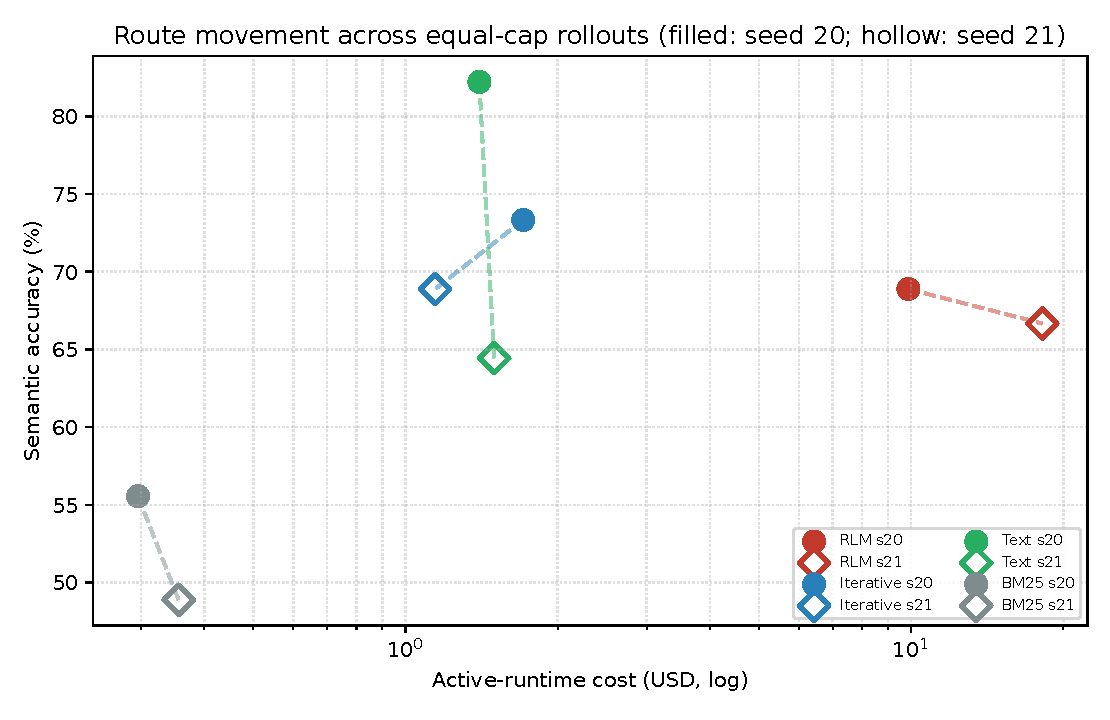
\includegraphics[width=0.98\linewidth]{figures_expansion/fig_pareto_dual_seed_overlay.pdf}
\caption{Equal-cap accuracy--cost movement across rollouts (filled markers:
prospective seed~20; hollow markers: post-hoc seed~21). Lines connect the same
route. Costs are route-attributed active runtime on a log axis. The plot does not
pool seeds into one estimator.}
\label{fig:supp-equal-cap-dual-seed}
\end{figure}

\begin{figure}[!htbp]
\centering
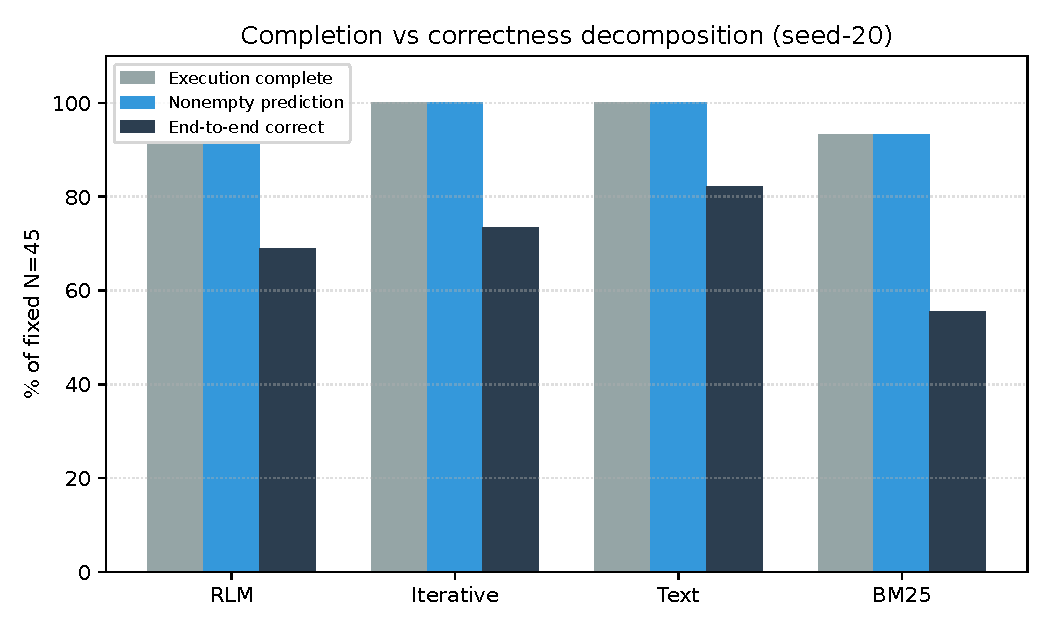
\includegraphics[width=0.98\linewidth]{figures_expansion/fig_completion_decomp_seed20.pdf}
\caption{Completion-versus-correctness decomposition on the prospective seed-20
endpoint: execution completion, nonempty prediction and end-to-end semantic
correctness under the fixed $N{=}45$ denominator. RLM's gap is concentrated in
completion and end-to-end correctness rather than empty predictions alone.}
\label{fig:supp-equal-cap-completion-decomp}
\end{figure}

These panels are descriptive re-analyses of the frozen equal-cap evidence. They
do not replace the Holm-controlled paired tests, do not add a prospective dense
full-pool route and do not authorize pooling seed~20 with seed~21.

\FloatBarrier
\subsection{Completion, Deadlines and Paired Rollout Sensitivity}
\label{app:completion-sensitivity}

These analyses reuse the 45 equal-cap queries and their two stored rollouts. They add no independent cases or model calls. All-case correctness keeps failed and invalid outputs in the denominator. Let $S$ be the queries for which every route returns a valid answer within 1,200 seconds. The selected comparison $|S|^{-1}\sum_{i\in S}(Y_{ir}-Y_{is})$ changes both the numerator and denominator. It is descriptive and cannot estimate what would have happened had an incomplete execution succeeded.

\begin{table}[htbp]
\centering
\small
\begin{tabular}{@{}llrrr@{}}
\toprule
Rollout & RLM minus & All 45 & Common completions & Change \\
\midrule
Seed 20 ($|S|=39$) & Iterative & $-4.4$ & $+5.1$ & $+9.6$ \\
 & Text & $-13.3$ & $-2.6$ & $+10.8$ \\
 & BM25 & $+13.3$ & $+20.5$ & $+7.2$ \\
Seed 21 ($|S|=34$) & Iterative & $-2.2$ & $+14.7$ & $+16.9$ \\
 & Text & $+2.2$ & $+23.5$ & $+21.3$ \\
 & BM25 & $+17.8$ & $+29.4$ & $+11.6$ \\
\bottomrule
\end{tabular}
\caption{Accuracy differences in percentage points. The last column is the change induced by restricting to common cap-valid completions, not a causal estimate of failure removal.}
\label{tab:selection-sensitivity}
\end{table}

The all-case difference decomposes without changing its denominator: $\widehat\Delta=45^{-1}\sum_{i\in S}(Y_{ir}-Y_{is})+45^{-1}\sum_{i\notin S}(Y_{ir}-Y_{is})$. For RLM versus iterative search in seed 21, the common-completion rows contribute $+5/45$, while excluded rows contribute $-6/45$, leaving $-1/45$ overall. This explains the sign reversal without imputing missing answers or attributing a causal effect to attrition.

A paired analysis of the change in route differences resamples query IDs jointly across both rollouts and both routes (50,000 bootstrap samples). The seed-21 minus seed-20 changes for RLM versus iterative, text and BM25 are respectively $+2.2$ points [$-22.2,26.7$], $+15.6$ [$-8.9,40.0$] and $+4.4$ [$-13.3,22.2$]. These post-hoc 95\% intervals describe case uncertainty conditional on two observed rollouts. They neither establish a seed-population interaction nor treat two measurements of one query as independent data.

\begin{figure}[htbp]
\centering
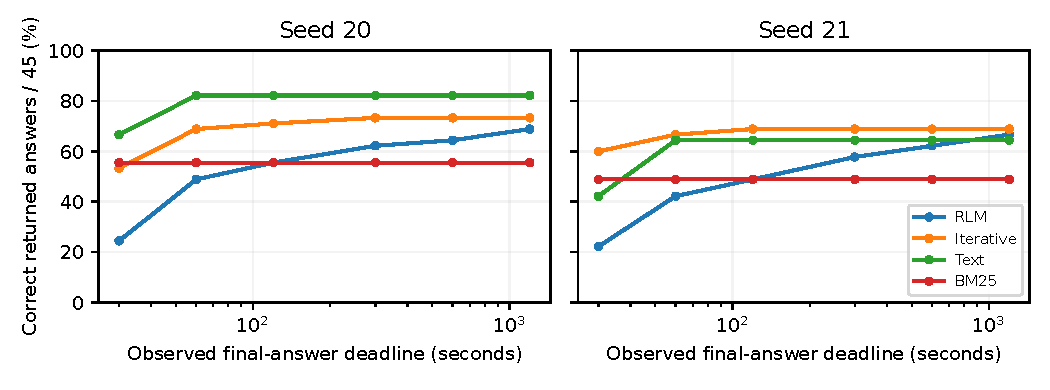
\includegraphics[width=\textwidth]{figures_expansion/observed_deadline_success.pdf}
\caption{Correct final answers returned by a given deadline on the retained runs, with all 45 queries in every denominator. The agent policy was held at its original cap: these are observed completion curves, not reruns with shorter instructed budgets. They exclude any unreturned intermediate answer and are not dollar-budget curves.}
\label{fig:observed-deadline}
\end{figure}

At 60 seconds, RLM/iterative/text/BM25 have returned 22/31/37/25 correct answers in seed 20 and 19/30/29/22 in seed 21. At 1,200 seconds the counts are 31/33/37/25 and 30/31/29/22. Longer allowed waiting reveals more correct RLM answers in these stored executions, while the relative ordering remains task- and rollout-specific. No confidence claim about fresh deployments is inferred from the curves alone.

\paragraph{Question-parser audit.}
The unchanged question parser was replayed using only the question string; the stored benchmark task and answer-type fields were used solely for checking agreement afterward. Both fields match on 150/150 SU-150 cases (73 context windows), 45/45 CD-45 cases (32 windows) and 45/45 VC-45 cases (20 windows), and every replay matches its original stored parser output. This repairs incomplete reporting of a check already represented in the stored outputs. It does not add new data or establish robustness to arbitrary paraphrases. In particular, selecting the correct task and answer type does not guarantee correct local labels, subset extraction, tie handling or the final answer.

The replay script writes per-case parser decisions, paired contrasts, exact McNemar tests with within-rollout Holm adjustment, selection decompositions, deadline counts and source hashes. Missing successful-output judgments, duplicate route/query cells and mismatched query IDs fail validation. All figures derive from the same analysis artifact.


\section{Repeatability and Cost Accounting}
\label{app:reproducibility}

\paragraph{Controlled families.}
T-STRUCT and the definitive T-MIXED $N=30$ comparison are single full-family passes. The T-MIXED old-finalizer run is a same-model $N=20$ mechanism probe; its exact-example manifest is reconstructed from stored model-I/O traces. The current-contract extension instead uses a separately frozen stable-generator manifest and SHA-256-derived offset, avoiding the historical generator's salted Python \texttt{hash(domain)} seed.

\paragraph{Public anchors.}
BrowseComp-Plus contributes four major estimates: the frozen $N=80$ two-episode completion, the zero-overlap score-blind attempted-$N=49$ replication stopped by its stability rule, the disjoint fixed-$N=45$ three-route replication with all 135 cells attempted before scoring and the prospective fixed-$N=45$ four-route equal-cap endpoint with all 180 cells attempted before scoring. The seed-21 rerun is a post-hoc same-row rollout sensitivity, not a fifth independent estimate. The earlier $N=37$ prefix records the first study's interruption and is not a confirmatory sample. T-NLP and T-SQ remain compatibility/proxy diagnostics; LB2 $>$500k and HotpotQA are bounded public diagnostics; and the public $\lambda$-RLM and prehend SRLM-style rows are pressure tests rather than official reproductions.

\paragraph{Cost accounting.}
Cost ratios compare routes within task families rather than through a global method denominator. RLM totals cover logged successful completions. The attempted-cost audit records their lower bound and the zero-usage failed rows that prevent exact reconstruction of partial failed-call billing.

\paragraph{Models and execution.}
Hosted models are identified by dated provider slug in the experiment records. The self-hosted BrowseComp endpoint uses Qwen3.6-35B-A3B-FP8 at a frozen weight revision and serving-image digest, a 65,536-token context limit, model-card decoding, disabled thinking and seed 20 (or 21 only for the labeled repeat). The official $\lambda$ row pins repository commit \texttt{3874d393483d}, weight revision \texttt{b968826d9c46} and \texttt{vllm/vllm-openai:v0.21.0} on one 80GB H100. The official trained-policy row uses an 80GB-class RunPod GPU and the canonical \texttt{rlm} harness at commit \texttt{72d6940142ddfb84e6be573dc999a37e633e671}.

\paragraph{Compute accounting.}
API experiments log returned tokens and list-price cost. Self-hosted BrowseComp costs use route-attributed active runtime at the recorded pod rate; generation-plus-judge totals are reported separately. Failed hosted calls sometimes return no usage, so attempted API cost is a lower bound. The complete official $\lambda$ CD-15 row required 6,562 seconds on one 80GB H100 and cost \$5.471 from creation through cleanup. The prospective seed-20 equal-cap endpoint attributes \$13.279 across route runtime and \$15.015 including the interrupted-episode lower bound and primary judging. The seed-21 repeat attributes \$21.170 across routes and \$22.374 from pod creation through primary judging and cleanup.

\paragraph{Data and release boundary.}
The study uses public or synthetic benchmark interfaces and does not redistribute source-document-scale BrowseComp-Plus, Oolong, LongBench-v2 or HotpotQA corpora. Access remains governed by upstream terms. The project retains frozen manifests, prompts, aggregate outputs, model-I/O traces, cost ledgers and deterministic claim verifiers. A public artifact is planned after anonymous review; the current single-PDF workshop submission makes no claim that code or data are already openly downloadable.

\FloatBarrier
\section{Reproducibility Commands}

\paragraph{Integrity and build commands.}
From the extracted release root, run \texttt{python3 verify\_release.py};
success is the final \texttt{ANONYMOUS RELEASE VERIFIER: PASS} line. This
deterministic command requires no network, model, API or GPU access.
